% Sample LaTeX file for creating a paper in the Morgan Kaufmannn two
% column, 8 1/2 by 11 inch proceedings format.

\documentclass[]{article}
\usepackage{uai2015stylefiles/proceed2e}

% Set the typeface to Times Roman
\usepackage{times}
\usepackage{amsmath, amssymb}
\usepackage{graphicx}
\usepackage{algpseudocode}
\usepackage{hyperref}
\usepackage{natbib}
\usepackage{color}
\usepackage{algorithm}
\usepackage{todonotes}

\definecolor{mydarkblue}{rgb}{0,0.08,0.45}
\hypersetup{ %
    pdftitle={},
    pdfauthor={},
    pdfsubject={},
    pdfkeywords={},
    pdfborder=0 0 0,
    pdfpagemode=UseNone,
    colorlinks=true,
    linkcolor=mydarkblue,
    citecolor=mydarkblue,
    filecolor=mydarkblue,
    urlcolor=mydarkblue,
    pdfview=FitH}

% Math typesetting.
\newcommand{\vx}{\mathbf{x}}
\newcommand{\vX}{\mathbf{X}}
\newcommand{\vw}{\mathbf{w}}
\newcommand{\vv}{\mathbf{v}}
\newcommand{\vr}{\mathbf{r}}
\newcommand{\vg}{\mathbf{g}}
\newcommand{\vI}{\mathbf{I}}
\newcommand{\vzero}{\bf{0}}
\newcommand{\ones}[1]{\mat{1}_{#1}}
\newcommand{\eye}[1]{\mat{E}_{#1}}
\newcommand{\tra}{^{\mathsf{T}}}
\newcommand{\vect}[1]{{\bf{#1}}}
\newcommand{\mat}[1]{\mathbf{#1}}
\newcommand{\pderiv}[2]{\frac{\partial #1}{\partial #2}}
\newcommand{\npderiv}[2]{\nicefrac{\partial #1}{\partial #2}}
\newcommand{\argmin}{\operatornamewithlimits{argmin}}
\newcommand{\argmax}{\operatornamewithlimits{argmax}}
\newcommand{\expect}{\mathbb{E}}
\newcommand{\expectargs}[2]{\mathbb{E}_{#1} \left[ {#2} \right]}
\newcommand{\var}{\mathbb{V}}
\newcommand{\varL}{\mathcal{L}}
\def\iid{i.i.d.\ }
\def\simiid{\overset{\mbox{\tiny iid}}{\sim}}
\newcommand{\defeq}{\mathrel{:\mkern-0.25mu=}}
\newcommand{\Normal}{\mathcal{N}}
\newcommand{\Nt}[3]{\mathcal{N}\!\left(#1 \middle| #2,#3\right)}
\newcommand{\N}[2]{\mathcal{N}\!\left(#1,#2\right)}
\DeclareMathOperator{\KLop}{KL}
\newcommand{\KL}[2]{\KLop \left(#1 \middle \| #2 \right)}

% Symbol definitions.
\newcommand{\distinit}{q_0(\params, \vv)}
\newcommand{\data}{\vx}

%% \newcommand{\params}{\vx}
\newcommand{\params}{\mathbf{\theta}}
\newcommand{\trans}{T}
\newcommand{\paramsrv}{\vX}  % Random variable.
\newcommand{\numsteps}{T}
\newcommand{\decay}{\gamma}
\newcommand{\decays}{{\boldsymbol{\decay}}}
\newcommand{\stepsize}{\alpha}
\newcommand{\stepsizes}{{\boldsymbol{\stepsize}}}
\newcommand{\gradparams}{\nabla L(\params_t, t)}
\DeclareMathOperator{\SGD}{SGD}
\newcommand{\entropy}{S}
\newcommand{\pun}{{\tilde p}}
\newcommand{\jointdist}{p(\params , \data)}
\newcommand{\posterior}{p(\params | \data)}
\newcommand{\subjointdist}[2]{p_{#1}(\params_{#2} , \data)}
\newcommand{\subjointdistminibatch}[1]{\tilde{p}(\params_{#1} , \data)}
\newcommand{\reals}{\mathbb{R}}
\newcommand{\bigo}[1]{\mathcal{O}\left(#1\right)}
\newcommand{\trace}[1]{\text{Tr}\left[#1\right]}
\newcommand{\loss}{L(\params)}

%\title{Maxwell's D\ae mon: Stochastic Gradient Nonparametric Variational Inference}
%\title{Entropic Descent: Stochastic Gradient Nonparametric Variational Inference}
%\title{Stochastic Gradient Descent is Nonparametric Variational Inference}
\title{Early Stopping is Nonparametric Variational Inference}

\author{} % LEAVE BLANK FOR ORIGINAL SUBMISSION.
          % UAI  reviewing is double-blind.

% The author names and affiliations should appear only in the accepted paper.
%
%\author{ {\bf Harry Q.~Bovik\thanks{Footnote for author to give an
%alternate address.}} \\
%Computer Science Dept. \\
%Cranberry University\\
%Pittsburgh, PA 15213 \\
%\And
%{\bf Coauthor}  \\
%Affiliation          \\
%Address \\
%\And
%{\bf Coauthor}   \\
%Affiliation \\
%Address    \\
%(if needed)\\
%}

\begin{document}

\maketitle

\begin{abstract}
We show that unconverged stochastic gradient descent and other popular optimization methods can be interpreted as procedures that generate samples from a nonparametric variational approximate posterior distribution.
This distribution is implicitly defined as the transformation of an initial distribution by a sequence of optimization updates into a final approximation.
Each step of the optimization results in an intermediate distribution and by keeping track of the changes in entropy over this sequence of distributions, we can form an unbiased estimator of the variational lower bound on the log marginal likelihood.
We can then maximize this bound with respect to the models' hyperparameters instead of using a separate validation set.
This Bayesian interpretation of SGD suggests improved overfitting-resistant optimization procedures and gives a theoretical foundation for popular tricks such as early stopping and ensembling.
Moreover, this procedure hints at a middle ground between point estimates arising from MAP inference, and fully-factored variational approximations.
\end{abstract}

\section{Introduction}

In much of machine learning, the central computational challenge is optimization; we try to minimize some training set loss with respect to a set of model parameters.
If we treat the training loss as a (negative) log-posterior, this amounts to searching for a maximum \emph{a posteriori} (MAP) solution.
Paradoxically, over-zealous optimization can yield worse test set results than incomplete optimization due to the phenomenon of \emph{over-training}.
A popular remedy to over-training is to invoke ``early stopping'' in which optimization is halted based on the continually monitored performance of the parameters on a separate validation set.
However, early stopping is both theoretically unsatisfying and incoherent from a research perspective: how can one rationally design better optimization methods if the goal is to achieve something ``powerful but not \emph{too} powerful''?
A related trick is to ensemble the results from multiple optimization runs from different starting positions.
Similarly, this must rely on imperfect optimization, since otherwise all optimization runs would reach the same optimum.

\begin{figure}[t]
\vskip 0.2in
\begin{center}
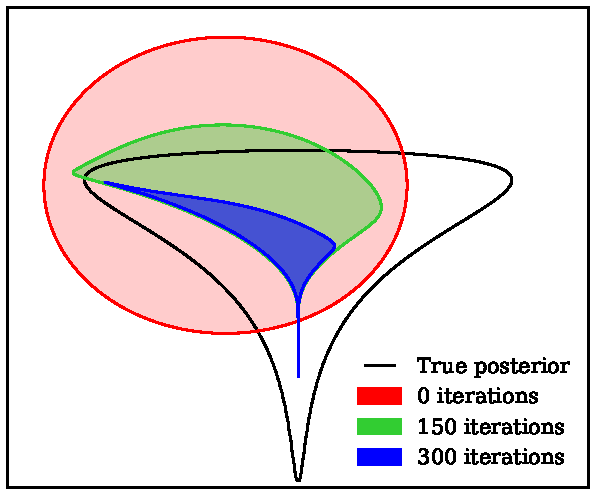
\includegraphics[width=\columnwidth]{../experiments/2015_03_02_funnel/2/dists.pdf}
\caption{A series of variational distributions implicitly defined by
  stochastic gradient descent on the log-likelihood.
  The initial distribution from which parameters are drawn (red) doesn't match the posterior (black).
  Intermediate distributions (green and blue) are implicitly defined by mapping each initial point through many iterations of gradient descent.
  These distributions don't have fixed parametric shapes, but depend on the shape of the entire posterior.}
\label{fig:cartoon}
\end{center}
\end{figure}

We propose an interpretation of incomplete optimization in terms of variational Bayesian inference.
Our starting point is a Bayesian posterior distribution for a potentially complicated model, in which there is an empirical loss that can be interpreted as a negative log likelihood and regularizers that have interpretations as priors.
One might proceed with MAP inference in such a setting and perform an optimization to find the best parameters.
The main idea of this paper is that such an optimization procedure, initialized according to some distribution that can be chosen freely, generates a sequence of distributions that are implicitly defined by the action of the optimization update rule on the previous distribution.
We can treat these distributions as variational approximations to the true posterior distribution.
A single optimization run for~$N$ iterations represents a draw from the~$N$th such distribution in the sequence.
For many popular optimization methods this sequence of distributions can be used to form an unbiased estimate of a lower bound on the log marginal likelihood.

With this interpretation, the number of optimization iterations can be seen as a variational parameter, one that trades off fitting the data well against maintaining a broad (high entropy) distribution.
Early stopping amounts to optimizing the variational lower bound (or an approximation based on a validation set) with respect to this variational parameter.
Similarly, since each optimization trajectory from a random initialization represents a sample from the variational distribution, ensembling random restarts can be viewed as building a sample-based approximation of (an approximation to) the posterior.

To establish whether this viewpoint is helpful in practice we ask (a)~whether we can estimate the marginal likelihood, and (b)~whether the family of variational distributions implied by the optimization rule yields a reasonably good approximation to the true posterior.
We tackle the first question in sections \ref{sec:techintro} and show that many popular optimization procedures yield tractable estimates of the marginal likelihood.
The second question is an empirical one, and we give some experimental evidence in both directions in section \ref{sec:experiments}.

\subsection{Contributions}
\begin{itemize}
\item We introduce a new interpretation of optimization algorithms as samplers from a variational distribution that adapts to the true posterior.
\item We provide a scalable estimator for the entropy of these implicit variational distributions, allowing us to estimate a lower bound on the marginal likelihood even on problems with millions of parameters.
\item We investigate the performance of these estimators empirically, and show that they have reasonable properties.
\end{itemize}

\section{Incomplete optimization as variational inference}
\label{sec:techintro}
Variational inference \citep{wainwright2008graphical} \todo{cite Hinton and possibly Ghahramani et al} aims to approximate an intractable posterior distribution, $\posterior$, with another distribution, $q(\params)$.
Ideally, the distribution~$q(\params)$ would belong to a simpler and tractable class, such as factored distributions or a parametric family.
The usual approach is to quantify the quality of the approximation using the Kullback-Leibler (KL) divergence from $q(\params)$ to $\jointdist$.
Such a measure also provides a lower bound on the marginal likelihood of the original model;
applying Bayes' rule to the definition of $\KL{q(\params)}{\posterior}$ gives the familiar inequality:
%
\begin{align}
\log p(\data)
& \geq - \underbrace{\expectargs{q(\params)}{ -\log \jointdist }}_{\textnormal{\normalsize Energy $E[q]$}}
         \underbrace{- \expectargs{q(\params)}{\log  q(\params)}}_{\textnormal{\normalsize Entropy $S[q]$}} \nonumber \\
& := \varL[q] \label{eq:varbound}
\end{align}
%
Maximizing $\varL[q]$, the variational lower bound on the marginal likelihood, with respect to $q$ minimizes $\KL{q(\params)}{\posterior}$, the KL divergence from $q$ to the true posterior, giving the closest approximation available within the variational family.
A convenient side effect is that we also get a lower bound on $p(\data)$, which can be used for model selection.

To perform variational inference, we require a family of distributions over which to maximize $\varL[q]$. 
Consider a general procedure to minimize the energy~$-\log\jointdist$ with respect to~${\params \in \reals^D}$.
The parameters~$\params$ are initialized according to some distribution~$q_0(\params)$ and updated at each iteration according to a transition operation~${\trans : \reals^D \rightarrow \reals^D}$:
%
\begin{align}
\params_0 &\sim q_0(\params) \nonumber \\
\params_{t + 1} &= \trans(\params_t), \nonumber
\end{align}
%
Our variational family consists of the sequence of distributions~$q_0, q_1, q_2, \ldots$,
where~$q_t(\params)$ is the distribution over~$\params_t$ generated by the above procedure.

As shown in (\ref{eq:varbound}), $\varL$ consists of an `energy' term and an `entropy' term.
The energy term measures how well~$q$ fits the data and the entropy term encourages the probability mass of~$q$ to spread out, preventing overfitting. \todo{not totally comfortable with the entropy term being about overfitting exactly}
As optimization of~$\params$ proceeds from its~$q_0$-distributed starting point, we can examine how~$\varL$ changes.
The negative energy term grows, since the goal of the optimization is to reduce the energy, while the entropy term shrinks, since the optimization converges over time.
Optimization thus generates a sequence of distributions that range from underfitting to overfitting, and the variational lower bound captures this tradeoff.

We cannot evaluate $\varL[q_t]$ exactly, but we can obtain an unbiased estimator.
Sampling~$\params_0$ from~$q_0$ and then applying the transition operator~$t$ times produces an exact sample~$\params_0$ from~$q_t$, by definition.
Since $\params_t$ is an exact sample from $q_t(\theta)$, $\log\subjointdist{}{t}$ is an unbiased estimator of the energy term of (\ref{eq:varbound}).
The entropy term is trickier, since we do not have access to the density $q(\params)$ directly.
However, if we know the entropy of the initial distribution, $S[q_0(\params)]$, then we can estimate $S[q_0(\params)]$ by looking at the change in entropy at each iteration, calculated by considering the change of variables formula for a probability density function.
To compute how the volume shrinks or expands due to this change of variables, we require access to the Jacobian of the optimizer's transition operator, $J(\params)$:
%
\begin{align}
S[q_{t+1}] - S[q_t] =
  \expectargs{q_t(\params_t)}{\log
    \left| J(\params_t) \right|} \,.
\end{align}
%
Note that this analysis assumes that the mapping $T$ is bijective.
Combining these terms, we have an unbiased estimator of $\varL$ at iteration $T$,
based on the sequence of parameters, $\params_0, \ldots, \params_T$, from a single training run.
\begin{align}
\varL[q_T] \approx
  \underbrace{\log \subjointdist{}{T}}_{\textnormal{\normalsize Energy}} +
  \underbrace{\sum_{t=0}^{T-1} \log \left| J(\params_t) \right| + S[q_0]}_{\textnormal{\normalsize Entropy}} \,.
\label{eq:entropy-bound}
\end{align}

\subsection{Stochastic Gradient Descent}

Stochastic gradient descent (SGD) is a popular and effective optimization procedure with the following update rule:
%
\begin{align}
\params_{t+1} &=
  \params_t - \stepsize \nabla \loss,
\end{align}
%
where the $\loss$ the objective loss (or an unbiased estimator of it e.g. using minibatches)
for example ~$-\log\jointdist$, and $\stepsize$ is a `step size' hyperparameter.
Taking the Jacobian of this update rule gives the following unbiased estimator
for the change in entropy at each iteration:
%
\begin{align}
S[q_{t+1}] - S[q_t] \approx \log \left| I - \stepsize H_t(\params_t)
\right| \label{eq:exact hessian}
\end{align}
%
where $H_t$ is the Hessian of $-\log\subjointdist{t}{}$ with respect to~$\params$.

Note that the Hessian does not need to be positive definite or even non-singular.
If some directions in $\params$ have negative curvature, the crest of a hill, it just means that optimization near there spreads out probability mass, increasing the entropy.
There are, however, restrictions on $\stepsize$.
If ${\stepsize\lambda_i = 1}$, for any $i$, where $\lambda_i$ are the eigenvalues of $H_t$, then the change in entropy will be undefined (infinitely negative).
Physically, this corresponds to a Newton-like update where multiple points collapse to the optimum in a single step giving a distribution with zero variance in a particular direction.
However, gradient descent is unstable anyway if ${\stepsize\lambda_{\text{max}} > 2}$, where~$\lambda_{\text{max}}$ is the largest eigenvalue of~$H_t$.
So if we choose a sufficiently conservative step size, such that $\stepsize\lambda_{\text{max}} < 1$,
this situation should not arise.

\begin{algorithm}[t]
   \caption{stochastic gradient descent with marginal likelihood estimate}
   \label{alg:sgd-with-estimate}
\begin{algorithmic}[1]
	\State {\bfseries input:}
	Weight initialization scale $\sigma_0$, step size $\stepsize$, 	
	twice-differentiable negative log likelihood $L(\params, t)$	
	\State {\bfseries initialize} $\params_1 \sim \N{0}{\sigma_0 \vI_D}$
	\State {\bfseries initialize} $\entropy_{1} = \frac{D}{2} (1 + \log 2 \pi) + D \log\sigma_0$
	\For{$t=1$ {\bfseries to} $T$}
%		\State $\vg = \gradparams$             \Comment{Evaluate gradient}
%		\State $\vr \sim \N{0}{\vI_D}$         \Comment{Draw random direction}
%		\State $\vr\tra \left[ -2 \vr + 3 \left(  R1 - R2 \right) \right]$      \Comment{Estimate determinant}
		\State $\entropy_{t+1} = \entropy_t - \log \left| \vI - \stepsize H_t \right|$  \Comment{Update entropy} \label{step:entropy-update}
		\State $\params_{t+1} = \params_t + \stepsize \gradparams$  \Comment{Update position}		
   \EndFor
   \State \textbf{output} sample $\params_T$, estimate of entropy $\entropy_T$
\end{algorithmic}
\end{algorithm}
%

So far, we have treated SGD as a deterministic procedure even though, as the name suggests,
the gradient of the loss at each iteration may be replaced by a stochastic version. Our analysis of the entropy is still if we fix the sequence of stochastic gradients to be the same for each optimization run, so that the only randomness comes from the parameter initialization.
This is a pedantic argument, similar to arguing that a pseudorandom sequence of numbers has only as much entropy as its seed.
However, if we do choose to randomize the gradient estimator differently for each training run
(e.g. choosing different minibatches) then the expression for the change in entropy, Equation \ref{eq:exact hessian}, remains valid as a \emph{lower bound} on the change in entropy and the 
subsequent calculation of $\varL$ remains a true lower bound on the log marginal likelihood.


\subsection{Estimating the Jacobian in high dimensions}
The expression for the change in entropy given by (\ref{eq:exact hessian}) is impractical for large-scale problems since it requires an~$\bigo{D^3}$ determinant computation.
Fortunately, we can make a good approximation using just one or two Hessian-vector products, which can usually be performed in~$\bigo{D}$ time using reverse-mode differentiation \citep{pearlmutter1994fast}.

The idea is that since~$\stepsize\lambda_{\text{max}}$ is small, the Jacobian is actually just a small perturbation to the identity and we can approximate its determinant using traces as follows:
%
\begin{align}
\log \left| I - \stepsize H \right|
& =    \sum_{i=0}^D \log\left(1 - \stepsize\lambda_i\right) \nonumber \\
& \geq \sum_{i=0}^D \left[- \stepsize\lambda_i 
                        - (\stepsize\lambda_i)^2 \right] \label{eq:logbound} \\
& = - \stepsize \trace{H} - \stepsize^2 \trace{HH}\,.
\end{align}
%
The bound in (\ref{eq:logbound}) is just a second order Taylor expansion of~$\log(1 - x)$ about~${x = 0}$ and is valid if ${\stepsize\lambda_i < 0.7}$. \todo{little o terms here for clarity?}
\todo{Mention closeness of bound.}
The trace of the Hessian can be estimated using inner products of random vectors
\citep{bai1996some}:
%
\begin{align}
\trace{H} = \expectargs{}{\vr^TH\vr}, \qquad \vr \sim \N{0}{I}\,.
\label{eq:approx-log-det}
\end{align}
%
A common problem, similar to the one we tackle here, is to compute the log of the determinant of the Hessian itself.
This arises, for example, in making the Laplace approximation to the posterior \citep{mackay1992practical}.
This is a much harder problem since the Hessian can be arbitrarily ill-conditioned, unlike our small Hessian-based perturbation to the identity.

Algorithm~\ref{alg:sgd-with-estimate} combines these steps into an algorithm that tracks the approximate entropy during optimization.
In high dimensions, the exact evaluation of the determinant in step~\ref{step:entropy-update} should be replaced with the approximation given by equation~\eqref{eq:approx-log-det}.


\subsection{Parameter initialization, priors, and objective functions}

What initial parameter distribution should we use for SGD?
The marginal likelihood estimate given by \eqref{eq:entropy-bound} is valid no matter which initial distribution we choose.
We could conceivably optimize this distribution in an outer loop using the marginal likelihood estimate itself.

However, using the prior distribution has several advantages.
First, it is usually designed to have broader support than the likelihood.
Since SGD usually decreases entropy, starting with a high-entropy distribution
is a good heuristic.

Another question we can ask is what to use as our objective loss. The obvious choice is the (unnormalized, negative) log-posterior but we can actually use any function we like.
The marginal likelihood estimate remains valid provided we can comptue its Hessian
(or appropriate Hessian vector products). A more sensible choice is to ignore the prior
in our SGD optimization and just take gradients and Hessians with respect to the log likelihood.
This way, if we use the prior to initialize the parameters, we only move away from this
initial distribution to the extent that the posterior differs from the prior.
This difference is just the log-likelihood.

\subsection{Designing entropy-friendly optimization methods}

The variational distribution implied by SGD does not optimize the variational lower bound directly.
If it happens to create a good variational distribution, it's only by accident.
In place of SGD, we can use any optimization method for which we can approximate the change in entropy, which in practice means any optimization for which we can compute Jacobian vector products.
Now that we have a variational interpretation of optimization we can start to design new 
optimization procedures with posterior-fitting in mind.

An obvious place to start is with stochastic update rule inspired by Markov Chain Monte Carlo (MCMC). 
Procedures like Hamiltonian Monte Carlo \citep{neal2011mcmc} and Langevin dynamics MCMC \citep{welling2011bayesian} look very much like optimiztion procedures but actually have the posterior as their stationary distribution.
This is exactly the approach taken by \citet{Bridging14}.
One difficulty with using stochastic updates, however, is that the calculating the change in
entropy at each iterationcan't requires access to the current distribution over parameters.
As an example, consider that convolving a delta function with a Gaussian yields an
infinite entropy increase, whereas convolving a uniform distribution with a Gaussian
yields no change in entropy. The authors \citep{welling2011bayesian} handle this
by learning a highly parameterized ``inverse model'' which implicitly models the distribution
over parameters. The downside of this is that the parameters of this model, which can be thought
of as variational parameters, must be learned in an outer loop.

Another, complementary approach, is to try to develop deterministic update rules
that avoid some of the pathologies of conventional update rules like sgd.
This could could be a research agenda in itself, but we give one example here of a modifcation to
sgd which can improve the variational lower bound.
One potential pathology of SGD in the context of posterior approximation, is that sgd can collapse the variational distribution into low-entropy filaments, shrinking in some directions to be orders of magnitude smaller than the width of the true posterior.
A simple trick to prevent this from happening is to apply a nonlinear, parameter-wise warping
to the gradient, such that directions of very small gradient do not get optimized all the way
to the optimium. For example,
%% \begin{align}

%% \end{align}
where $\g_0$ is a parameter that sets the scale of this shrinkage. Computing the Jacobian
of this new update rule gives a new rule to update the entropy estimate.
%% \begin{align}

%% \end{align}
The effect is that entropy is not removed from parameters which are sufficiently close to the optimum. An experiment showing the effect of this modified sgd is shown in Figure \cite{fig:cartoon-fatter}.

\begin{figure}[h]
\vskip 0.2in
\begin{center}
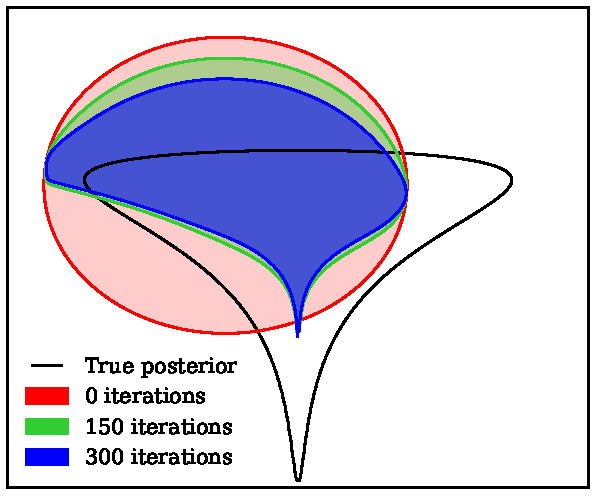
\includegraphics[width=\columnwidth]{../experiments/2015_03_02_funnel/3_grad_threshold/dists.pdf}
\caption{The variational distribution implied by the modified SGD algorithm.
Compared to Figure \ref{fig:cartoon}, the variational distributions are slower to collapse into low-entropy filaments.}
\label{fig:cartoon-fatter}
\end{center}
\end{figure}

\section{Experiments}
\label{sec:experiments}

In this section we show that the marginal likelihood estimate can be used to choose when to stop training, to choose model capacity, and to optimize training hyperparameters without the need for a validation set.
We are not attempting to motivate SGD variational inference as a superior alternative to other procedures. 
We simply wish to give a proof of concept that the marginal likelihood estimator has reasonable properties.

%\subsection{Boston housing data}
\subsection{Choosing when to stop optimization}

As a simple demonstration of the usefulness of our marginal likelihood estimate, we show that it can be used to estimate the optimal number of training iterations before overfitting begins.
We performed regression on the Boston housing dataset 
%[citation needed]
using a neural network with 100 hidden units, and no regularization.

\begin{figure}[h!]
%\vskip 0.2in
\begin{center}
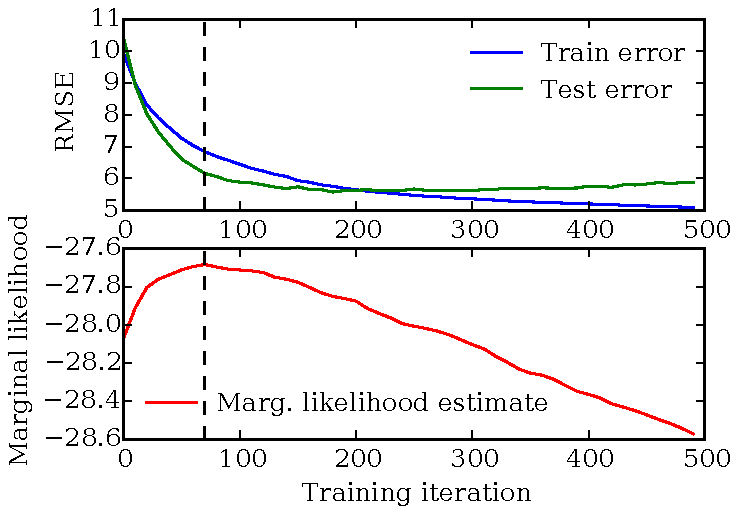
\includegraphics[width=\columnwidth]{../experiments/2015_03_01_housing/2/marglik}
\vskip -0.1in
\caption{\emph{Top}: Training and test-set error on the Boston housing dataset.
\emph{Bottom}: Marginal likelihood estimate.
The dashed line indicates the iteration with highest marginal likelihood.
The marginal likelihood, estimated online using only the training set, has a maximum at an iteration close to when the test error is best.}
\label{fig:housing}
\end{center}
\end{figure}


Figure \ref{fig:housing} shows overfitting and show marginal likelihood peaks at a similar place to the peak of held-out log-likelihood.

%\subsection{MNIST handwritten digits}
\subsection{Choosing the number of hidden units}

%(Show that noiseless version doesn't perform particularly well. Noise does a good job with the overfitting problem. But does can we capture the marginal likelood well? Do we need to do AIS to check?)

The marginal likelihood estimate is also comparable between training runs, allowing us to use it to select model hyperparameters, such as the number of hidden units.

\begin{figure}[h!]
%\vskip 0.2in
\begin{center}
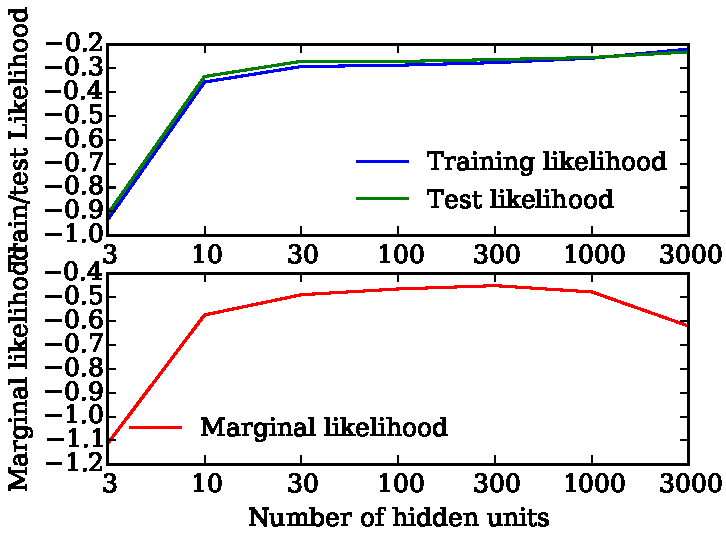
\includegraphics[width=\columnwidth]{../experiments/2015_03_03_vary_width/6_hidden_units/vary_widths.pdf}
\vskip -0.1in
\caption{\emph{Top}: Training and test-set likelihood as a function of the number of hidden units in the first layer of a network.
\emph{Bottom}: Marginal likelihood estimates.}
\label{fig:num hiddens}
\end{center}
\end{figure}

Figure \ref{fig:num hiddens} shows marginal likelihood estimates as a function of the number of hidden units in the first hidden layer of a 3-layer deep neural network, trained on 50000 MNIST handwritten digits.



\subsection{Optimizing training hyperparameters}

We can also use marginal likelihoods to optimize training parameters such as learning rates, or initial distributions.
As an example, Figure \ref{fig:threshold} shows the marginal likelihood estimate as a function of the gradient threshold in the modified SGD algorithm, again trained on 50000 MNIST handwritten digits.

\begin{figure}[h!]
%\vskip 0.2in
\begin{center}
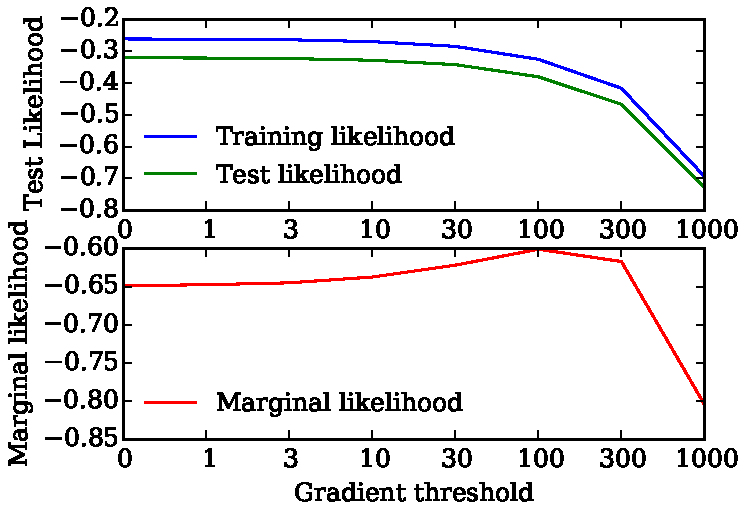
\includegraphics[width=\columnwidth]{../experiments/2015_03_03_vary_width/5_grad_threshold/vary_widths.pdf}
\vskip -0.1in
\caption{\emph{Top}: Training and test-set likelihood as a function of the gradient threshold.
\emph{Bottom}: Marginal likelihood as a function of the gradient threshold.
A gradient threshold of zero corresponds to standard SGD.}
\label{fig:threshold}
\end{center}
\end{figure}

As the level of thresholding increases, training and test error get worse due to under-fitting.
However, for intermediate thresholds, the lower bound increases.
Because it is a lower bound, its increase means that the estimate of the marginal likelihood is becoming \emph{more accurate}, even though the actual model happens to be getting worse at the same time.



\section{Limitations}

Estimating marginal likelihood is known to be sharp-P hard in general.
When do we expect the estimate of the marginal likelihood to be poor?




\section{Related work}

\paragraph{Early stopping}
Stein's unbiased risk estimator (SURE)~\citep{stein1981estimation} provides an unbiased estimate of generalization performance under very broad conditions.
\citet{raskutti2014early} derived a SURE estimate for SGD.
Interestingly, this estimator depends on the `shrinkage matrix' $\prod_{t=0}^{T} ( \vI - \stepsize_t H_T )$, which is just the Jacobian of the entire SGD procedure along a particular path.
However, this estimator depends on an estimate of the variance of noise variance, and does not provide a lower bound.

\citet{raskutti2014early} also derive a data-dependent early-stopping rule for kernel regression methods, but it not clear whether this stopping rule could be adapted to arbitrary twice-differentiable models, or whether it could be used to select all training and model hyperparameters.




\paragraph{Reversible learning} 
Optimization is an
intrinsically information-destroying process, since a (good) optimization
procedure maps any initial starting point to one or a few final optima. We can
quantify this loss of information by asking how many bits must be stored in order
to reverse the optimization, as in \citet{MacDuvAda2015hyper}.
 We can think of this as average the number of bits
`learned' during the optimization.

From this perspective, stopping before optimization
converges can be seen as a way to limit the number of bits we try to learn,
since we don't expect to be able to learn more than a finite number of bits from a finite dataset.

Thus, early stopping can also be seen as one of many ways to reduce the hypothesis space to improve generalization.
% (cite MDL? Statistical learning theory?)

\paragraph{MCMC for variational inference}
Our method can be seen as a special case of \citet{Bridging14}, who showed that any set of stochastic dynamics, even those not satisfying detailed balance, can be used to implicitly define a variational distribution.
However, to provide a tight variational bound, one needs to estimate the entropy of the resulting implicit distribution.
\citet{Bridging14} do this by defining an inverse model which estimates backwards transition probabilities, and then optimizes this model in an outer loop.
In contrast, our dynamics are deterministic, and our estimate of the entropy has a simple fixed form.


\paragraph{Bayesian neural networks}
Variational inference in Bayesian neural-network models such as deep Gaussian processes~\citep{deepGPVar14}.
\citet{kingma2014efficient} show how neural networks having unknown weights can be reformulated as neural networks having known weights but stochastic hidden units, and exploit this connection to preform efficient gradient-based inference in Bayesian neural networks.


\paragraph{Black-box stochastic variational inference}
\citet{alp2014blackbox} introduce a general scheme for variational inference using only the gradients of the log-likelihood of a model.
However, they constrain their variational approximation to be Gaussian, as opposed to our free-form variational distribution.

%\paragraph{Adaptive learning rates for SGD}
%\citet{courbariaux2014low} give a method based on Hessian-vector products to adapt learning rates for stochastic gradient descent without momentum.



%\paragraph{Annealed HMC}
%\citet{sohl2012hamiltonian} used HMC including an accept/reject step for annealed importance sampling to estimate partition functions.

%\paragraph{HMC with fewer rejections}
%\citet{sohl2014hamiltonian} introduce a variant of HMC that requires fewer rejections by extending trajectories in some cases where a rejection would otherwise occur, giving a sampler that does not obey detailed balance but still samples from the correct stationary distribution.

%\paragraph{MCMC with mini batches}
%[TODO: more citations go here]
%\citet{betancourt2015fundamental} argues that minibatches are fundamentally incompatible with HMC.


\section{Future Work and Extensions}

\paragraph{Optimization with momentum}
One obvious extension would be to design an estimator of the entropy lost by momentum-based optimizers such as stochastic gradient descent with momentum, or Adam~\citep{Adam14}.
However, it is difficult to track the entropy change during the updates to the momentum variables.

We could derive a variational inference algorithm based on RMSprop~\cite{Tieleman2012}, and a corresponding variant of Hamiltonian Monte Carlo.

\paragraph{Gradient-based hyperparameter optimization}
Hyperparameters typically come in two forms:
Regularization parameters and training parameters.
Optimizing marginal likelihood rather than training loss lets us set regularization parameters during training without using a validation set.
The marginal likelihood estimate lets us optimize the variational parameters (training hyperparameters) in an outer loop.
However, optimizing more than a few of these is difficult without gradients.
We could gain access to exact gradients of the variational lower bound with respect to all variational parameters by simply using reverse-mode differentiation.
\citet{MacDuvAda2015hyper} showed that this can be done in a memory-efficient way for momentum-based learning procedures.
Combining these two procedures would allow one to set all hyperparameters using gradient-based methods without the need for a validation set.

\paragraph{Stochastic dynamics}
One possible method to deal with over-zealous reduction in entropy by SGD would be to add noise to the dynamics.
In the case of Gaussian noise, we would recover Langevin dynamics.
However, estimating the entropy becomes much more difficult in this case.
\citet{welling2011bayesian} introduced stochastic gradient Langevin dynamics for doing inference with minibatches.
\citet{ma2013estimating} use Langevin dynamics and a floating temperature to estimate partition functions of graphical models.
%\citet{vollmer2015non} analyze the asymptotics of Langevin dynamics.

More generally, we are free to design optimization algorithms that do a better job of producing samples from the true posterior, as long as we can track their entropy.
The gradient-thresholding method proposed in this paper is a simple first example of a refinement to SGD that maintains a tractable entropy estimate while improving the quality of the intermediate distributions.



\section{Conclusions}

Optimization algorithms with random initializations implicitly define a series of distributions which converge to posterior modes.
We showed that these nonparametric distributions can be seen as variational approximations to the true posterior, when the optimization objective is a log-likelihood.
We showed how to produce an unbiased estimate of this variational lower bound by approximately tracking the entropy.
This simple and inexpensive calculation turns standard gradient descent into an inference algorithm, and allows the optimization of hyperparameters without a validation set.
Our estimate is compatible with using data minibatches, and scales linearly with the number of parameters, making it suitable to large-scale problems.




%or optimizers that handle different parameters more gracefull, are parameterization-invariant etc.

%\subsection{Acknowledgements}
%We thank Roger Grosse for helpful discussions. Also Miguel and Matt Johnson, and Oren Rippel.




\bibliography{references.bib}
\bibliographystyle{uai2015stylefiles/icml2015}

\end{document}

% ==============================================================================


\begin{figure}
%\vskip 0.2in
\begin{center}
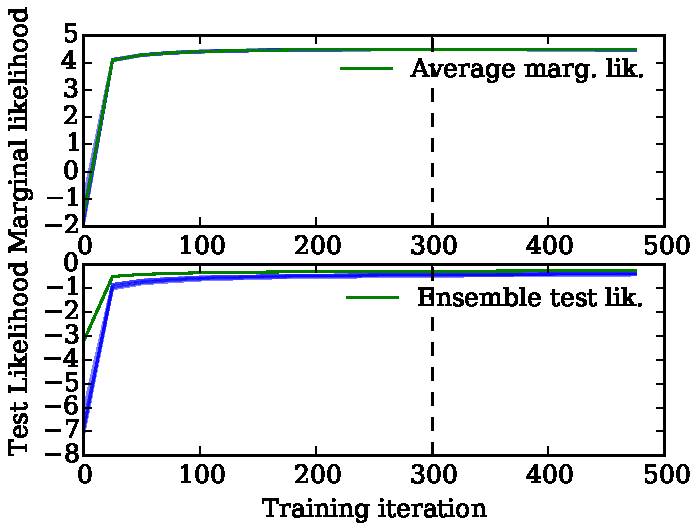
\includegraphics[width=\columnwidth]{../experiments/2015_02_27_first_entropic_sgd/6_ensemble/ensemble}
\vskip -0.1in
\caption{\emph{Top}: Marginal likelihood estimate.
\emph{Bottom}: Test-set error on the MNIST dataset.}
\label{fig:ensemble}
\end{center}
\end{figure}

Figure \ref{fig:ensemble} shows...

\subsection{Adding noise to increase entropy}
(Adding noise is the obvious way to increase entropy. If noise variance is
exactly double step size then this is just stochastic langevin dynamic (cite
Welling and Teh) and if we're doing MCMC then this is just like bridging the gap
paper. But the hard part is now estimating entropy. It requires an estimate of q
itself but we don't have access to q directly. Luckily, any q will do, it will
just be a looser bound if we get it wrong. The approach of Welling et al is
to make a parametric form which is learned. We propose a simpler approach. We
expect it to eventually converge to the true posterior, and we know the initial
distribution. So we approximate as it goes along with a convex combination of
these two log probs. Annealing so that we're actaully targeting these as we go
along is another possiblity.)

(Maybe mention that treating sgd as a deterministic procedure is a bit
disingenuous: it might be formally deterministic but the selection of
minibatches is certainly arbitrary. Perhaps you could get better performance by
formalizing the randomness and accounting for it.)



We define a nonparametric variational distribution implicitly as the output of a
random initialization run through $T$ iterations of stochastic gradient descent
(SGD):

%
\begin{align}
\params_1, \vv_1 & \sim \distinit \\
q^{\SGD}_T(\params, \vv) & = \SGD(\stepsizes, \decays, \params_1, \vv_1, T)
\end{align}
%

\subsection{Leapfrog Dynamics}

In the limit of small step sizes $\stepsize$, leapfrog dynamics exactly preserve the energy and entropy of the system, and therefore the marginal likelihood of the implicit variational distribution remains the same.

No matter the step size, leapfrog dynamics always exactly preserve entropy.
The only time entropy is added or removed from the system is when the momentum is resampled.
The difference in this entropy is given by:
%
\begin{align}
\Delta H & = H_t' - H_t \\
 & = - \expectargs{q_(\vx)}{\expect_{q'(\vv|\vx)} \log q'(\vv|\vx) - \expect_{q(\vv|\vx)} \log q(\vv|\vx)} \nonumber \\
 & = - \expect{q_(\vx)} \Bigg[ \expect_{q'(\vv|\vx)} \log q'(\vv|\vx) - \expect_{q(\vv|\vx)} \log r(\vv|\vx) \nonumber \\ 
 & \quad - \underbrace{\expect_{q(\vv|\vx)} \log \frac{ q(\vv|\vx)}{r(\vv|\vx)}}_{\textnormal{\scriptsize $\KL{q(\vv|\vx)}{r(\vv|\vx)}$}} \Bigg] \label{eq:r slack}
\end{align}
%

In the case of SGD with momentum, entropy is lost only when drag is applied.
If the momentum is decayed by $\vv_{t+1} = \decay_t \vv_t$, then the amount of entropy lost is exactly $\log \decay$.

\begin{figure}[t]
%\vskip 0.2in
\begin{center}
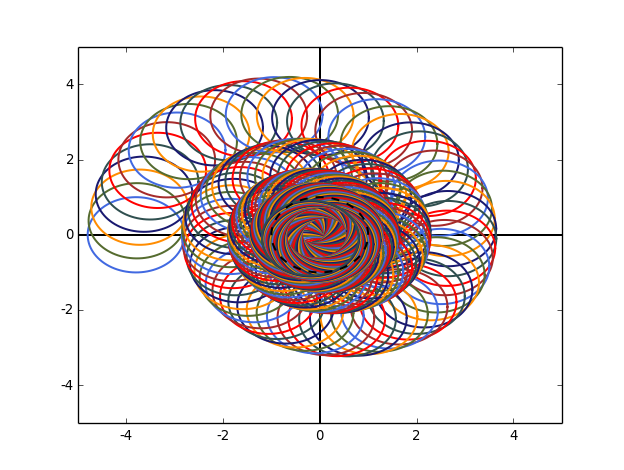
\includegraphics[width=\columnwidth]{../experiments/2015_02_23_gaussian_phase_diagrams/1/phase_diagram}
\caption{Phase diagram over time.}
\label{fig:phase}
\end{center}
\end{figure}


\begin{algorithm}
   \caption{Entropic Descent}
   \label{alg:entropic-descent}
\begin{algorithmic}[1]
	\State {\bfseries input:}
	Weight initialization scale $\sigma_0$, \\
	velocity randomization level $\decay$, \\
	annealing schedule $\stepsizes$, \\
	time step $\epsilon$, \\
	highest eigenvalue $\lambda$, \\
	negative log likelihood $L(\params, t)$
	\State initialize $\vv_1 \sim \N{0}{\vI_D}$
	\State initialize $\params_1 \sim \N{0}{\sigma_0 \vI_D}$
	\State $\entropy = \frac{D}{2} (1 + \log 2 \pi) + D \log\sigma_0 + \frac{1}{2} (D - |\vv|_2^2)$
	\For{$t=1$ {\bfseries to} $T$}
		\State $\entropy = \entropy + \frac{1}{2} |\vv|_2^2$ \Comment{Update entropy}
		\State $d =   \stepsizes_t \lambda     + (1 - \stepsizes_t) \sigma_0^2$ \Comment{Anneal stepsize}
		\State $\vg = \stepsizes_t \gradparams + (1 - \stepsizes_t) \frac{\vx}{\sigma_0^2}$ \Comment{Anneal gradient}
		\State $\vv_{t+1} = \vv_t + d \times \vg$ \Comment{Update velocity}
		\State $\params_{t+1} = \params_t + d \times \vv$  \Comment{Update position}
		\State $\entropy = \entropy - \frac{1}{2} |\vv|_2^2$  \Comment{Downdate entropy}
		\State $\vr \sim \N{0}{\vI_D}$
		\State $d\vv = \sqrt{1 - \decay^2} d\vv + \decay \vr$ \Comment{Perturb velocity}
   \EndFor
   \State \textbf{output} sample $\params_T$, estimate of entropy $\entropy$
\end{algorithmic}
\end{algorithm}

$\lambda$ is the square root of the highest eigenvalue of the Hessian of the log-posterior at the mode.
$\decay$ controls the amount velocities randomize each iteration.

Since we can sample exactly from $q$, we can approximate the first (``energy'') term of $L$ using one or more Monte Carlo samples.

The variational parameters of $q^{\SGD}$ are the learning rate schedule $\stepsizes$, the momentum decay schedule $\decays$ and the initial distribution $\distinit$.
Perhaps for now we'll set $\distinit$ to be the prior, although it could really be anything.

\subsection{The need for Annealing}
If we didn't anneal, the KL term in equation \ref{eq:r slack} wouldn't go to zero even as the step-size approached zero.

\subsection{But what about detailed balance?}



\begin{figure*}[t]
%\vskip 0.2in
\begin{center}
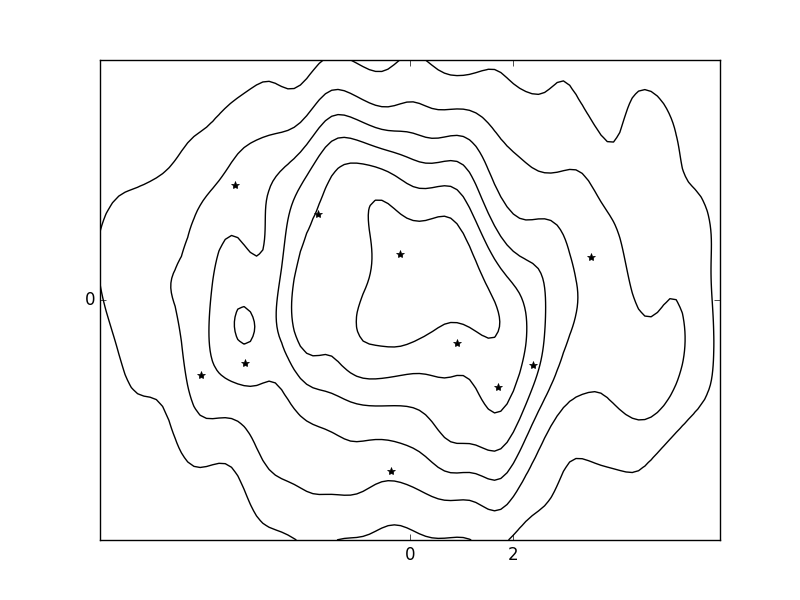
\includegraphics[width=0.18\linewidth]{../experiments/2015_02_19_caibration/5_figure/seqs/densities_0}
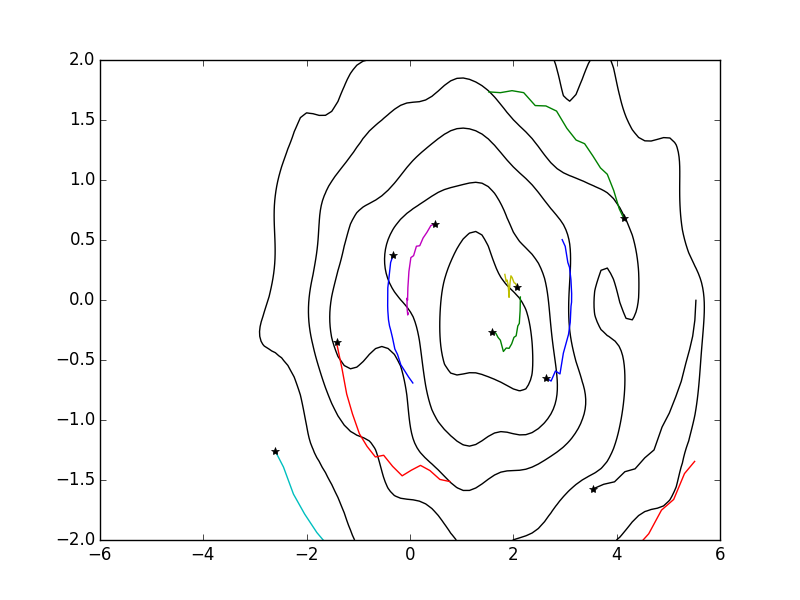
\includegraphics[width=0.18\linewidth]{../experiments/2015_02_19_caibration/5_figure/seqs/densities_200}
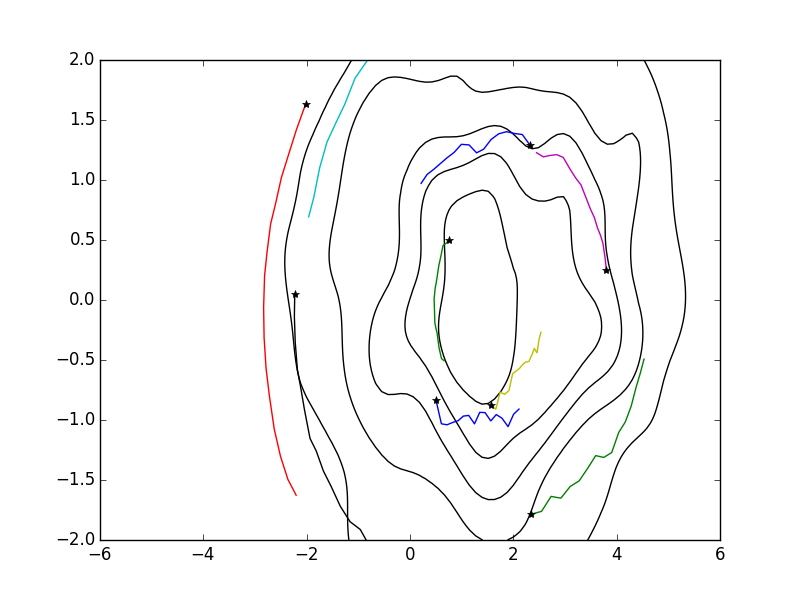
\includegraphics[width=0.18\linewidth]{../experiments/2015_02_19_caibration/5_figure/seqs/densities_400}
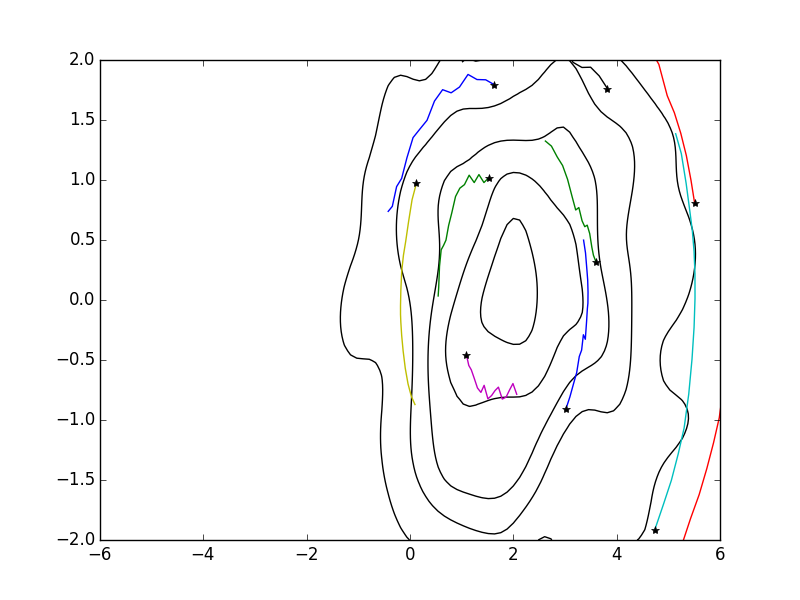
\includegraphics[width=0.18\linewidth]{../experiments/2015_02_19_caibration/5_figure/seqs/densities_600}
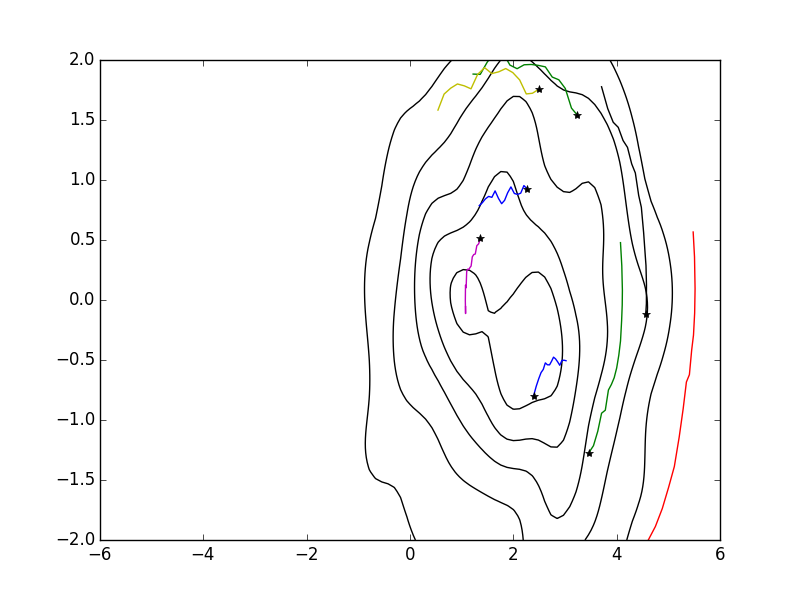
\includegraphics[width=0.18\linewidth]{../experiments/2015_02_19_caibration/5_figure/seqs/densities_800}
\caption{Left to right: Phase diagrams over time.}
\label{fig:dynamics}
\end{center}
\end{figure*}



\section{Online gradient updates of learning rate and momentum}

A simple procedure to sample from a variational posterior could look like this:
Start with $\stepsize_1 = 1$, $\decay_1 = 1$.
At each iteration of SGD, update each in the direction that would improve the bound at computed at the current step,~$L_{t+1}$:
%
\begin{align}
\vv_{t+1}     & = \decay_t \vv_t - g(\params_t) \\
\params_{t+1} & = \params_t + \stepsize_t \vv_{t+1} \\
\stepsize_{t+1} & = \stepsize_t + s_\stepsize \pderiv{L_t}{\stepsize_t} \\
\decay_{t+1} & = \decay_t + s_\decay \pderiv{L_t}{\decay_t}
\end{align}
%
where $s_\stepsize$ and $s_\decay$ are `meta' step sizes.

Which direction do these gradients point?
For $\stepsize$,
%
\begin{align}
\pderiv{L_t}{\stepsize_t} = g(\params_{t+1}) \vv_{t+1}
\end{align}
%
which means that the learning rate will increase as long as the gradient is pointing in the same direction as the velocity.
It also has the effect of going at the same speed when the gradient becomes small.
This is what we want:  If learning stopped when the gradient was zero, then the optimizer would converge.

For $\decay$, the gradient has the form:
%
\begin{align}
\pderiv{L_t}{\decay_t} = - g(\params_{t+1}) \vv_{t} \stepsize_t - \log \decay_t
\end{align}
%
The first term is exactly the same as our heuristic, scaled by $\stepsize$!
It will increase the velocity if the gradient points in the opposite direction from the velocity.

The second term has a damping effect:  If the gradient, velocity, or stepsize are all small, then this term will try to set the momentum decay term to 1.
When the momentum decay term is exactly one, no entropy is lost or gained by the optimizer.


How to optimize the variational parameters $\stepsizes$ and $\decays$?
Keep in mind that these could be different for every iteration of SGD as well as every parameter.
Keep in mind that since our approximation to the lower bound is deterministic in $\stepsizes$ and $\decays$, we can easily ``overfit'' the variational hyperparameters unless we average over multiple runs of SGD. [TODO: this doesn't have to be the case. It depends on whether we can reversibly infer the momentum decay rate as we go along.]

\section{Online gradient updates of learning rate and momentum}

A simple procedure to sample from a variational posterior could look like this:
Start with $\stepsize_1 = 1$, $\decay_1 = 1$.
At each iteration of SGD, update each in the direction that would improve the bound at computed at the current step,~$L_{t+1}$:
%
\begin{align}
\vv_{t+1}     & = \decay_t \vv_t - g(\params_t) \\
\params_{t+1} & = \params_t + \stepsize_t \vv_{t+1} \\
\stepsize_{t+1} & = \stepsize_t + s_\stepsize \pderiv{L_t}{\stepsize_t} \\
\decay_{t+1} & = \decay_t + s_\decay \pderiv{L_t}{\decay_t}
\end{align}
%
where $s_\stepsize$ and $s_\decay$ are `meta' step sizes.

Which direction do these gradients point?
For $\stepsize$,
%
\begin{align}
\pderiv{L_t}{\stepsize_t} = g(\params_{t+1}) \vv_{t+1}
\end{align}
%
which means that the learning rate will increase as long as the gradient is pointing in the same direction as the velocity.
It also has the effect of going at the same speed when the gradient becomes small.
This is what we want:  If learning stopped when the gradient was zero, then the optimizer would converge.

For $\decay$, the gradient has the form:
%
\begin{align}
\pderiv{L_t}{\decay_t} = - g(\params_{t+1}) \vv_{t} \stepsize_t - \log \decay_t
\end{align}
%
The first term is exactly the same as our heuristic, scaled by $\stepsize$!
It will increase the velocity if the gradient points in the opposite direction from the velocity.

The second term has a damping effect:  If the gradient, velocity, or stepsize are all small, then this term will try to set the momentum decay term to 1.
When the momentum decay term is exactly one, no entropy is lost or gained by the optimizer.

Taken together, these two update rules mean that when the local gradient goes to zero, the velocity will stabilize and not go to zero, and the stepsize will also remain constant.
This is also necessary for the optimizer not to stop at local minima.
These dynamics will also skate over basins at a constant speed, which is what we want.

[TODO] see if there are any other steady states of this system, such as going in a circle around the minimum of a parabola.

No burn in!

\section{Reversibility}

We can probably play with the order of the SGD steps to make them reversible.
But do we need to?
If we interpret $\stepsizes$ and $\decays$ as just variational parameters, then they are "outside" the system, and the only way they can go wrong is by failing to find a good bound, or by messing up our estimates of the bound.

\section{Alternative approach - decay rate from velocity variance estimate}

If we treat $\decays$ as variational parameters we have to use the same
$\decays$ regardless of starting position and trajectory. Some smoothing will
therefore be necessary to avoid overfitting to a perticular trajectory. If we
evaluate multiple trajectories from an ensemble of starting positions, we can
chose $\decay$ based on the statistical properties of this ensemble.

In particular, we happen to know the target distribution's marginal distribution
over $\vv$ (it's just $N(0, 1)$ independent of $\params$).  The purpose of the
decay term is to collapse the velocity towards this distribution.  We can
estimate the variance, $\sigma_v^2$, of the variational distribution over $\vv$
at time $T$ using the ensemble and then, for example, choose:
\begin{align}
\log \decay = - \beta_0 \log \sigma_v
\end{align}
For some overall ``decay speed'' $\beta_0$. [TODO: think about the multivariate
case, in which $\decays$ could be a matrix. With $N << D$ samples, we can't
hope to estimate the full covariance matrix. Maybe some ones on the diagonal
would help.]

\section{Alternative approach - decay rate adapted using curvature information}

If we base $\decays$ entirely on $\params$ and not on $\vv$ we can have
different $\decays$ for different trajectories and we don't have to worry about
overfitting.

If we have a good estimate of the entropy difference between initial and target
distributions we can choose some integrable $\decays$ schedule that amortizes
the entropy change over multiple steps. The log determinant of the Hessian is
such an estimate. It's exact in the Gaussian case and hopefully a reasonable
approximation otherwise. Looking at the individual eigenvalues of the Hessian
gives a way to estimate the required entropy injection/extraction along each
eigendirection.

[TODO: think about how to avoid actually diagonalizing the Hessian]

[TODO: think about how to handle negative eigenvalues]

\section{Yet another approach - velocity randomization}

An orthonormal transformation of the velocity vector leaves the target
distribution invariant and the entropy unchanged. So if we just apply a
transformation of $I + \alpha T$ at each iteration, we will get a similar effect
to that of a per-parameter $\decay$, without having to devise an elaborate
heuristic to assign a $\decay$ to each parameter. There is just one global
$\decay$ which controls the overall rate of entropy extraction and the remaining
entropy is automatically distributed among the parameters as needed by the
random rotations.

This is a lot like randomizing velocities in the manner of HMC, except that it
doesn't add or remove any net entropy. Entropy is only added or removed when we
apply $\decay$ for which we are rewarded or penalized as appropriate.

------

Since we can sample exactly from $q$, we can approximate the first (``energy'') term of $L$ using one or more Monte Carlo samples.
We can compute the second (``entropy'') term exactly:
\begin{align}
S[q_t] = S[q_0] - \sum_{t=1}^{T} \sum_{d=1}^{D} \log \decay_{td}
\end{align}
%
where $f(\params)$ is the negative log-likelihood and $\decay_{td}$ is the velocity decay rate for step $t$ and parameter $d$.
[Maybe: mention that it's only a lower bound on the entropy in the case of finite precision.]

(Planning to test out how well it performs in practice. Not claiming it's the
best thing ever. Just scientifically interested in how good of an approximation
it is.)

In general, what do we most care about in this section?
\begin{itemize}
\item Quality of marginal likelihood estiamte
\item Quality of approximating distribution
\item Comparison between marginal likelihood estimate and held-out likelihood
\item Slackness of bound due to imperfect guessing of distribution when using
  noisy/mcmc version
\item Quality of Hessian randomized trace estimate
\item Noisiness of stochastic estimates
\end{itemize}

